\chapter{Deployment}
\label{chap:deployment}

\section{Automated Unity Builds using Unity Cloud Build}
While Unity and Git don't necessarily work too well together out of the box as mentioned in Section~\ref{sec:unityGit} one might start to wonder whether automatic build processing is possible. Having a central hub with automatically built binaries can be quite useful for testing the game and providing the correct binaries for testers. Unity offers a free service called \emph{Unity Cloud Build} which provides this functionality. 

\begin{figure}[tbph]  %t top, b bottom, p page | you can also use h to try to get the figure to appear at the current location
  \centering
  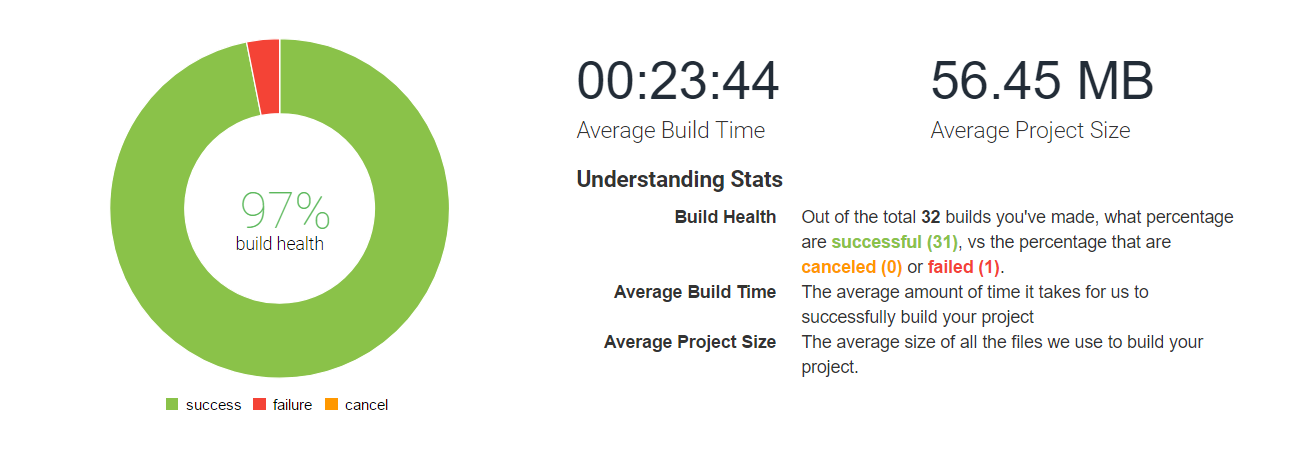
\includegraphics[width=\textwidth]{images/unityCloudBuildStats}
  \caption[Project statistics from Unity Cloud Build]{Unity Cloud Build's project statistics illustrate the status of the build process.}
  \label{fig:unityCloudStats}
\end{figure}

Unity Cloud Build allows the developer to set up automatic builds for different target platforms and integrates with BitBucket using SSH keys to get access to the project repository. Specific branches to be built can be specified directly within the service and provides shareable links which can be given to others for both deployment and testing purposes. The service also offers build statistics as seen in Figure~\ref{fig:unityCloudStats} and allows for automatic execution of specific unit tests. 

We have integrated our BitBucket repository with Unity Cloud Build to make sure that we always have an up to date build available for Windows, MacOS and Linux. 

\subsection{Dockit League binaries}
This Section contains the binaries for the game which are built at the time of thesis hand in through the use of Unity Cloud Build's shared links. In order to download the latest build of \emph{Dockit League} we recommend visiting the BitBucket repository~\cite{bitbucketRepo} and downloading the binaries from the links on the front page. There is no necessary installation needed when downloading the game as the downloaded folder includes all the files for the game. 

These are the links to the different builds:
\begin{itemize}
    \item Windows x86:  \cite{x86build}
    \item Windows x64:  \cite{x64build}
    \item macOS:  \cite{macOSbuild}
    \item Linux:  \cite{linuxbuild}
\end{itemize}